% This example An LaTeX document showing how to use the l3proj class to
% write your report. Use pdflatex and bibtex to process the file, creating 
% a PDF file as output (there is no need to use dvips when using pdflatex).

% Modified 

\documentclass{l3proj}
\begin{document}
\title{Team R Project Dissertation}
\author{Alex Chilikov \\
        Jacob Ford \\
        Mike Harling \\
        Ivaylo Lafchiev \\
        Mindaugas Ribikauskas \\
        Akos Szente}
\date{1 March 2016}
\maketitle
\educationalconsent
\tableofcontents
%==============================================================================
\chapter{Introduction}
\label{intro}

An introduction, explaining the purpose of the document, a very brief outline of the project and a summary of the structure of the rest of the document (approximately 1-2 pages).

The following text illustrates how to cite and input figures.

ALICE \cite{alice} was beginning to get very tired of sitting by her sister
on the bank and of having nothing to do: once or twice she had peeped into
the book her sister was reading, but it had no pictures or conversations in
it, ``and what is the use of a book,'' thought Alice, ``without pictures or
conversations?'

So she was considering, in her own mind (as well as she could, for the hot
day made her feel very sleepy and stupid), whether the pleasure of making a
daisy-chain would be worth the trouble of getting up and picking the
daisies, when suddenly a White Rabbit with pink eyes ran close by her.

There was nothing so very remarkable in that; nor did Alice think it so
very much out of the way to hear the Rabbit say to itself ``Oh dear! Oh
dear! I shall be too late!'' (when she thought it over afterwards it
occurred to her that she ought to have wondered at this, but at the time it
all seemed quite natural); but, when the Rabbit actually took a watch out
of its waistcoat-pocket, and looked at it, and then hurried on, Alice
started to her feet, for it flashed across her mind that she had never
before seen a rabbit with either a waistcoat-pocket, or a watch to take out
of it, and burning with curiosity, she ran across the field after it, and
was just in time to see it pop down a large rabbit-hole under the hedge.

In another moment down went Alice after it, never once considering how in
the world she was to get out again.

The rabbit-hole went straight on like a tunnel for some way, and then
dipped suddenly down, so suddenly that Alice had not a moment to think
about stopping herself before she found herself falling down what seemed to
be a very deep well.

Either the well was very deep, or she fell very slowly, for she had plenty
of time as she went down to look about her, and to wonder what was going to
happen next. First, she tried to look down and make out what she was coming
to, but it was too dark to see anything: then she looked at the sides of
the well, and noticed that they were filled with cupboards and
book-shelves: here and there she saw maps and pictures hung upon pegs. She
took down ajar from one of the shelves as she passed: it was labeled
``ORANGE MARMALADE'' but to her great disappointment it was empty: she did
not like to drop the jar, for fear of killing somebody underneath, so
managed to put it into one of the cupboards as she fell past it.

``Well!'' thought Alice to herself ``After such a fall as this, I shall think
nothing of tumbling down-stairs! How brave they'll all think me at home!
Why, I wouldn't say anything about it, even if I fell off the top of the
house!'' (which was very likely true.)

Down, down, down. Would the fall never come to an end? ``I wonder how many
miles I've fallen by this time?'' she said aloud. ``I must be getting
somewhere near the centre of the earth. Let me see: that would be four
thousand miles down, I think-'' (for, you see, Alice had learnt several
things of this sort in her lessons in the school-room, and though this was
not a very good opportunity for showing off her knowledge, as there was no
one to listen to her, still it was good practice to say it over) `` yes
that's about the right distance -- but then I wonder what Latitude or
Longitude I've got to?'' (Alice had not the slightest idea what Latitude
was, or Longitude either, but she thought they were nice grand words to
say.)

Presently she began again. ``I wonder if I shall fall fight through the
earth! How funny it'll seem to come out among the people that walk with
their heads downwards! The antipathies, I think-'' (she was rather glad
there was no one listening, this time, as it didn't sound at all the right
word) ``but I shall have to ask them what the name of the country is, you
know. Please, Ma'am, is this New Zealand? Or Australia?'' (and she tried to
curtsey as she spoke- fancy, curtseying as you're falling through the air!
Do you think you could manage it?) ``And what an ignorant little girl she'll
think me for asking! No, it'll never do to ask: perhaps I shall see it
written up somewhere.''

Down, down, down. There was nothing else to do, so Alice soon began talking
again. ``Dinah'll miss me very much to-night, I should think!'' (Dinah was
the cat.) ``I hope they'll remember her saucer of milk at tea-time. Dinah,
my dear! I wish you were down here with me! There are no mice in the air,
I'm afraid, but you might catch a bat, and that's very like a mouse, you
know. But do cats eat bats, I wonder?'' And here Alice began to get rather
sleepy, and went on saying to herself, in a dreamy son of way, ``Do cats eat
bats? Do cats eat bats?'' and sometimes ``Do bats eat cats?'' for, you see, as
she couldn't answer either question, it didn't much matter which way she
put it. She felt that she was dozing off, and had just begun to dream that
she was walking hand in hand with Dinah, and was saying to her, very
earnestly, ``Now, Dinah, tell me the truth: did you ever eat a bat?'' when
suddenly, thump! thump! down she came upon a heap of sticks and dry leaves,
and the fall was over.

Alice was not a bit hurt, and she jumped up on to her feet in a moment: she
looked up, but it was all dark overhead: before her was another long
passage, and the White Rabbit was still in sight, hurrying down it. There
was not a moment to be lost: away went Alice like the wind, and was just in
time to hear it say, as it turned a comer, ``Oh my ears and whiskers, how
late it's getting!'' She was close behind it when she turned the comer, but
the Rabbit was no longer to be seen: she found herself in a long, low hall,
which was lit up by a row of lamps hanging from the roof.

There were doors all round the hall, but they were all locked; and when
Alice had been all the way down one side and up the other, trying every
door, she walked sadly down the middle, wondering how she was ever to get
out again.

Suddenly she came upon a little three-legged table, all made of solid
glass: there was nothing on it but a tiny golden key, and Alice's first
idea was that this might belong to one of the doors of the hall; but, alas!
either the locks were too large, or the key was too small, but at any rate
it would not open any of them. However, on the second time round, she came
upon a low curtain she had not noticed before, and behind it was a little
door about fifteen inches high: she tried the little golden key in the
lock, and to her great delight it fitte!d

\begin{figure}
\begin{center}
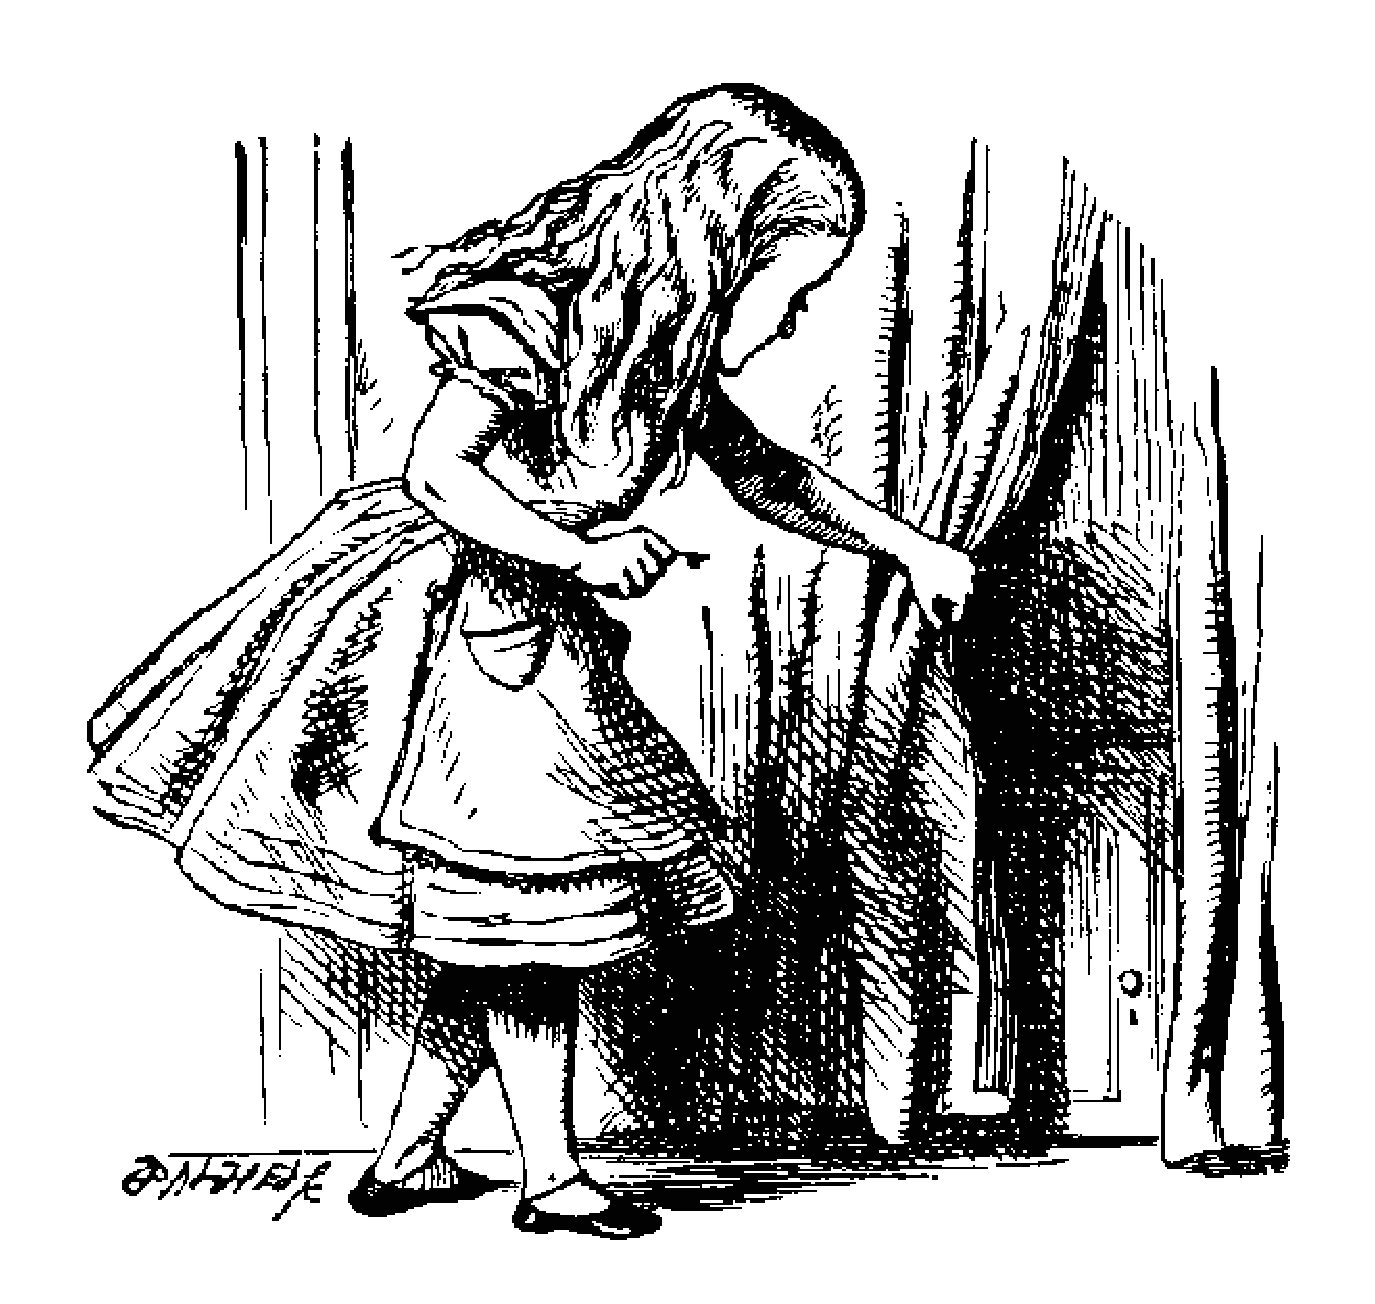
\includegraphics[width=7cm]{figures/alice}
\end{center}
\caption{Behind it was a little door}
\label{fig:alice}
\end{figure}

Alice opened the door and found that it led into a small passage, not much
larger than a rat-hole: she knelt down and looked along the passage into
the loveliest garden you ever saw. How she longed to get out of that dark
hall, and wander about among those beds of bright flowers and those cool
fountains, but she could not even get her head through the doorway; ``and
even if my head would go through,'' thought poor Alice, ``it would be of very
little use without my shoulders. Oh, how I wish I could shut up like a
telescope! I think I could, if I only knew how to begin.'' For, you see, so
many out-of-the- way things had happened lately, that Alice had begun to
think that very few things indeed were really impossible.

There seemed to be no use in waiting by the little door, so she went back
to the table, half hoping she might find another key on it, or at any rate
a book of rules for shutting people up like telescopes: this time she found
a little bottle on it, (``which certainly was not here before,'' said Alice),
and tied round the neck of the bottle was a paper label, with the words
``DRINK ME'' beautifully printed on it in large letters.It was all very well
to say ``Drink me,'' but the wise little Alice was not going to do that in a
hurry. ``No, I'll look first,'' she said, ``and see whether it's marked
'poison' or not''; for she had read several nice little stories about
children who had got burnt, and eaten up by wild beasts, and other
unpleasant things, all because they would not remember the simple rules
their friends had taught them: such as, that a red-hot poker will burn you
if you hold it too long; and that, if you cut your finger very deeply with
a knife, it usually bleeds; and she had never forgotten that, if you drink
much from a bottle marked ``poison,'' it is almost certain to disagree with
you, sooner or later.However, this bottle was not marked ``poison,'' so Alice
ventured to taste it, and, finding it very nice (it had, in fact, a sort of
mixed flavour of cherry-tart, custard, pine-apple, roast turkey, toffy, and
hot buttered toast), she very soon finished it off.

``What a curious feeling!'' said Alice. ``I must be shutting up like a
telescope!''

And so it was indeed: she was now only ten inches high, and her face
brightened up at the thought that she was now the right size for going
through the little door into that lovely garden. First, however, she waited
for a few minutes to see if she was going to shrink any further: she felt a
little nervous about this; ``for it might end, you know,'' said Alice to
herself; ``in my going out altogether, like a candle. I wonder what I should
be like then?'' And she tried to fancy what the flame of a candle looks like
after the candle is blown out, for she could not remember ever having seen
such a thing.

After a while, finding that nothing more happened, she decided on going
into the garden at once; but, alas for poor Alice! when she got to the
door, she found she had forgotten the little golden key, and when she went
back to the table for it, she found she could not possibly reach it: she
could see it quite plainly through the glass, and she tried her best to
climb up one of the legs of the table, but it was too slippery; and when
she had tired herself out with trying, the poor little thing sat down and
cried.

``Come, there's no use in crying like that!'' said Alice to herself rather
sharply. ``I advise you to leave off this minute!'' She generally gave
herself very good advice (though she very seldom followed it), and
sometimes she scolded herself so severely as to bring tears into her eyes;
and once she remembered trying to box her own ears for having cheated
herself in a game of croquet she was playing against herself, for this
curious child was very fond of pretending to be two people. ``But it's no
use now,'' thought poor Alice, ``to pretend to be two people! Why, there's
hardly enough of me left to make one respectable person!''

Soon her eye fell on a little glass box that was lying under the table: she
opened it, and found in it a very small cake, on which the words ``EAT ME''
were beautifully marked in currants. ``Well, I'll eat it,'' said Alice, ``and
if it makes me grow larger, I can reach the key; and if it makes me grow
smaller, I can creep under the door: so either way I'll get into the
garden, and I don't care which happens!''

She ate a little bit, and said anxiously to herself ``Which way? Which
way?'', holding her hand on the top of her head to feel which way it was
growing; and she was quite surprised to find that she remained the same
size. To be sure, this is what generally happens when one eats cake; but
Alice had got so much into the way of expecting nothing but out-of-the-way
things to happen, that it seemed quite dull and stupid for life to go on in
the common way.

So she set to work, and very soon finished off the cake. 

%==============================================================================
\chapter{Case Study}
\label{case}

A description of the case study background and context. This should include a description of the project customer (what was the nature of the organisation you were working for), their objectives for the project, and a summary of what was actually achieved. Where appropriate, this section should also make reference to similar related projects in order to make the context clear (approximately 4-5 pages).

%==============================================================================
\chapter{Reflections}


\section{The premature design decision}
\label{design}

(alex-note - introduction of the reflection - what it is about and summarizing what we will talk about
-the issue
-practices used
-what we learned
-our experience during the process
)
The first reflection we would like to discuss as part of the reflection chapter is about the premature design decisions which were made as part of our software engineering process, the practices we used, and what we learned and changed about them as a result of the difficulties we experienced during the process.

(Introduce the reflection better explain the situation )
The premature design decision refers to the fact that both the front and back ends of the application were develop to expect separate execution paths for different deprivation criteria.(introduction of reflection) The reason for implementing both parts in this way was as initially it was considered that each deprivation criterion can have different data related to it and different search parameters, potentially distinctive analyser (justification of mistake). This justification can lead us to several possible paths for a  discussion.

(justification why  it was expected different deprivation criteria to have different data
-assumptions
-probable misunderstanding
-lack of thorough documentation
-bad initial requirements gathering
-meeting only 30 minutes
)
Firstly, the different data related to different criteria was an assumption made by the team at the begining of the application processes. Most likely, as it was later discussed with the teammates, this was due to the fact that this requirement was not initially discussed with the client, an often observed situnation in which software developers make premature design desicions caused as a result of misunderstanding or introducing of an assumption either from the client or the software development team later significantly affecting the project (QUOTE)(premature assumptions and misunderstanding duing an initial meeting). Another potential reason is the lack of thorough documentation at the beginning of the software process. The lack of such documentation lead to the hiding of the assumption which could have been potentially avoided if an appropriate thorough documentation was present to reveal it(initial lack of documentation - maybe QUOTE). A third potential explanation for the trouble can be explored as part of the initial requirements gathering activity(bad initial requirements gathering - quoute). A more complete requirements elicitation with regard to the type of data expected could have potentially prevented the issue. If we had investigated what data exactly we could expect for each of the deprivation criteria during the meeting, such a misunderstanding could have been avoided. Furthermore, the lack of time, due to the limitation of the 30 minute initial meeting is an additional explanation we can analyse as a cause. A possible way for preventing it is an improvement of the communication between the team and the client using more frequent exchanges of emails.

(expect different search criteria for different criteria)
Secondly, the presence of different search parameters for different deprivation criteria was another argument to use different work flows for each deprivation criterion. This later turned out to be a wrong assumption, as some of the potential reasons for this can be identified in the following alternatives. Perhaps the most significant of the them is the lack of understanding of the project and more precisely what can be expected from a benchmarking tool from the point of view of the client. One way for avoid this in future project is potentially presenting prototypes(quote- why this is good) or expecting from the client to show us other projects as closely related to what he expects as possible(quote). Alternatively, a further reading about the project objectives would have additionally contributed for avoiding such mistakes in future (quote).

(different analyser)
The final potential reason for the expected separate work flows for each deprivation criterion can be found in the expectation of different analysers. The analysers are the classes responsible for the business logic of the back end, they provide the estimates for a particular deprivation criterion selection. It was not initially known what type(ies) of statistical distribution(s) will be used, whether the users will be able to choose them and correspondingly if they will be allowed to modify the confidence interval.  All of these assumptions were not well considered and were not realized as assumptions instead it was simply considered that this should be the expected way the application to be done providing this functionality, which later was discovered not to be the case. A potetial edifying conclusion of these facts can be that prior planning is important and that the project development team should have first better identify the requirements, clarify and discuss them for confirmation with the customer instead of making premature assumption. It would have been better if the time spend coding at the begining of the design process was spent better understanding and planning the scope of the application.

(impact)
In this paragraph the impact of the premature design decision will be discussed. Once the reasons for its manifesting were identified and it was explained, the complete impact of the decison will help the reader better understand why the particular decisions were take to deal with the situation. First, one of the major impacts were the cost related to implementing the separate work paths for each of the deprivation criteria. This lead to repetition of code both in the front and back end when this time could have been better spent for resolving other tasks. Additionally to this, the increased number of classes in the back end needed more thorough testing (a test for each class) which similarly was a repetition of code and waste of time for the team. Finally, the use of separate execution paths for different deprivation criteria lead to increased complexity and consequtively more expensive maintance.

Fortunately, the premature design decision even leading to the negative impact described above had positive effects as well. It introduced a trade-off between complexity and time related cost and flexibility, opportunities for improvement and easier maintanence. In this paragraph the advantages of the decision are presented. Firstly, as stated above the overall flexibility of project was improved as a result of the premature design decidsion it made it possible different Analyser classes to me introduced for different deprivation criteria to allow their estimation to be handled separately in case we have different data for different deprivation criteria which even if it is not the case now can potentially be in the future. This is particularly important fact as the application is a heavily related to its data - it is a benchmarking tool, so flexibility related to different analysers is extremely useful feature. More specifically, each of the analysers can use a different statistical distibution equation based on the different type of deprivation criteria for providing more accurate results for providing reliable estimates which can be the only case for some deprivation criteria and data distributions. As an example, if a new deprivation criterion is introducted with limited data the current uniform distribution schema is not a suitable probabilistic solution. In such a scenario other distribution equations must be adopted. As discussed with the client, there is a long list of additional parameters required from him which will not be implemented as part of the current release due to the lack of time. Secondly, the use of different execution paths provides alternative search mechanisms and parameters. More specifically, using subparamaters for different deprivation criteria is a possible extra search mechanism refining the search and providing more flexibility as part of an advance search for example. The idea of subparameters appear as part of the final product but is left a "read-only" functionality which is not functioning at the moment because of the lack of more precise data and sources such a a more precise data can be imported from.

(What changed in the project team (if anything) as a result of the experience?)
aus
As a final part of this reflection, we would like to present the changes we did as part of our software engineering processing as a result of the experience. First, we significantly improved our interviewing processes meeting in advance and discussing what we will talk during the meetings presenting our progress, which was allowing any assumption to be identified in time and prevented before they become a considerable part of the application. Additionally, we adopted a practice to document all of our meetings with the client and disucss our understing of the new features to be implemented during the next iteration cycle. As a proof of this you can look at the team R moodle page. The complete documentation of meetings made it  possible to better understand what it is expected from us. As a particularly appropriate example we can look at the second interview documentation wiki. There two sections there which are particularly relevant, namely ALGORITHM FOR OUTPUT and COMMENTARY ON PROTOTYPE. The algorithm for output section explains in detail the way the analyser classes from above must be designed and resolve potential issues with assumptions related to using more than one analyser, different confidence intervals, and distribution equations making it clear how the estimation must function to prevent introduction of further assumption. The second section the COMMENTARY ON PROTOTYPE refers to the prototype we created to similarly decrease the number of assumptions, premature design decision and the cost associated with them. The prototype was particularly useful way prevent premature design decisions with respect to the front end in particular. Additionall, documenting the feedback given from the client for the prototype made it straightforward to confirm his expectations about the front end and later design and implement it feelng confident that our implementation is what is expected and desired by the customer.

To conclude this reflection, the premature design decision lead to additional work and following financial cost related to this. They were mainly caused by poor documentation, assumptions, and bad interview practices. All of this potential causes were limited using prototypes for removing assumptions and getting approval by the client, improved documentation and better interview methadologies. Overally, the premature design decisions provided a great amount of flexibility as well such as opportunity for adding alternative distribution equations, different confidence intervals, and deprivation criteria subparameters. In brief, the premature design decisons caused some potential difficulties but they helped us learn a lot and improve our software engineering process as supported by the arguments above.
 
 


%==============================================================================
\section{Implementation}
\label{impl}

In this chapter, we describe how the implemented the system.

%------------------------------------------------------------------------------
\section{User Interface}

Blah blah blah
Blah blah blah
Blah blah blah
Blah blah blah

% - - - - - - - - - - - - - - - - - - - - - - - - - - - - - - - - - - - - - - -
\subsection{Foo}

Blah blah blah
Blah blah blah
Blah blah blah
Blah blah blah

%------------------------------------------------------------------------------
\section{Database Model}

\begin{enumerate}
\item Blah blah blah
\item Blah blah blah
\item Blah blah blah
\item Blah blah blah
\end{enumerate}



%==============================================================================
\section{Evaluation}

We evaluated the project by...

%==============================================================================
\chapter{Conclusion}

A conclusion that draws general and wider lessons from the case study (approximately 1-2 pages).

%==============================================================================
\section{Contributions}

Here we explain that Lewis Carroll wrote chapter \ref{intro}. John Wayne
was out riding his horse every day and didn't do anything. Marilyn Monroe
was great at getting the requirements specification and coordinating the
writing of the report. Betty Davis did the coding of the kernel of the
project, described in Chapter \ref{impl}.  James Dean handled the
multimedia content of the project.

%==============================================================================
\bibliographystyle{plain}
\bibliography{example}
\end{document}
